\clearpage
\section*{Index Construction}
\phantomsection
\addcontentsline{toc}{section}{Index Construction}

% ============================================================================ 
% TERM WEIGHTING
% ============================================================================ 
\subsection*{Term Weighting Definition}
\phantomsection
\addcontentsline{toc}{subsection}{Term Weighting Definition}

Our codebase evaluates four distinct term weighting methodologies with 
third-party libraries and custom mathematical implementations.

Term frequency and inverse document frequency (TF-IDF) are calculated globally 
during the instantiation of the \texttt{DataProcessing} class. 
\texttt{TfidfVectorizer} normalizes the document vectors to a uniform length, 
regardless of the original document's size. Then, at query time, the
\texttt{VSMSearch} class applies the \texttt{vectorizer.transform()} function 
to the query string. This function call converts the query text into a 
numerical matrix. We then compute the retrieval scores using the
\texttt{cosine\_similarity()} metric against the pre-computed, sparse matrix. 

Our BM25 implementation delegates the complex mathematics to the 
\texttt{rank-bm25} library. We initialize the \texttt{BM250kapi} class with 
an array of tokenized document arrays. Query execution is then handled natively 
by passing the tokenized query array into the \texttt{.get\_scores()} function.
This function call outputs an array of probabilistic scores that correspond 
to the exact original document indices. 

The BIM algorithm utilizes our custom-built scoring function, 
\texttt{\_bim\_score()}, that evaluates term presence. The algorithm does this 
by mapping each document to a Python \texttt{set} for distinct vocabulary 
extraction. The weight of a query term is then calculated dynamically with the 
following formula:
$$\text{Score} = \sum_{t \in Q \cap D} \log \Bigg(\frac{N-n_i+0.5}
{n_i+0.5}\Bigg),$$
where $N$ is extracted from the length of the \texttt{doc\_ids} and $n_i$ 
is retrieved from our pre-computed document frequency dictionary.

Our unigram and bigram Language Models are implemented manually for 
strict control of probability interpolation. The functions
\texttt{\_unigram\_score} and \texttt{\_bigram\_score} map the probabilities 
to $\log$ space, summing the results. This algorithm prevents zero-probabilities 
by linearly interpolating the local maximum likelihood estimate and the 
collection probability using a static smoothing parameter, $\lambda$. To 
calculate for the probability that a document $D$ is relevant to a query 
term $t$, the following formula was implemented:
$$\mathcal{P}(t|D) = \lambda \Bigg(\frac{tf_{t,d}}{L_d}\Bigg) + (1-\lambda) 
\Bigg(\frac{cf_t}{L_c}\Bigg),$$
where $\lambda$ is the smoothing parameter statically set to $0.3$, $tf_{t,d}$ 
is the term frequency of a document, $L_d$ is the length of a document, 
$cf_t$ is the collection frequency (i.e., how many times does the specific 
query term appear across the entire database of documents), and $L_c$ is the 
length of the collection (i.e., what is the total number of words in the entire 
database).

% ============================================================================ 
% INDEX DESIGN
% ============================================================================ 
\subsection*{Index Design}
\phantomsection
\addcontentsline{toc}{subsection}{Index Design}

The foundation for our retrieval system's index design begins with utilizing 
the \texttt{pandas} library to read from the provided JSON dataset 
collection. This transforms the dataset to data frame objects within our 
\texttt{DataProcessing} class. Relevance judgments are aggregated using 
vectorized operations to optimize the evaluation phase. In other words, 
this transformed the tabular data into an efficient dictionary of 
\texttt{set} objects which enable $\mathcal{O}(1)$ lookups for relevant 
document verification during precision calculations. Furthermore, 
our system builds separate indexes dictated by the specific requirements 
of the retrieval models. 

For the Vector Space Model, the index is constructed as a \textit{Compressed
Sparse Row (CSR)} matrix using \texttt{TfidfVectorizer}. This variant of the 
index abstracts the vocabulary mapping, storing the mathematical weights in 
memory for optimized matrix dot-products. 

For our models that require fine frequency calculations (e.g., BIM and 
Language Models), the index is designed using hash maps. Our system constructs 
unigram and bigram term-frequency mappings. This design similarly allows for 
$\mathcal{O}(1)$ retrieval of local documents lengths, collection occurrences, 
and document frequencies required for probabilistic scoring. 

\begin{figure}[htbp]
    \centering
    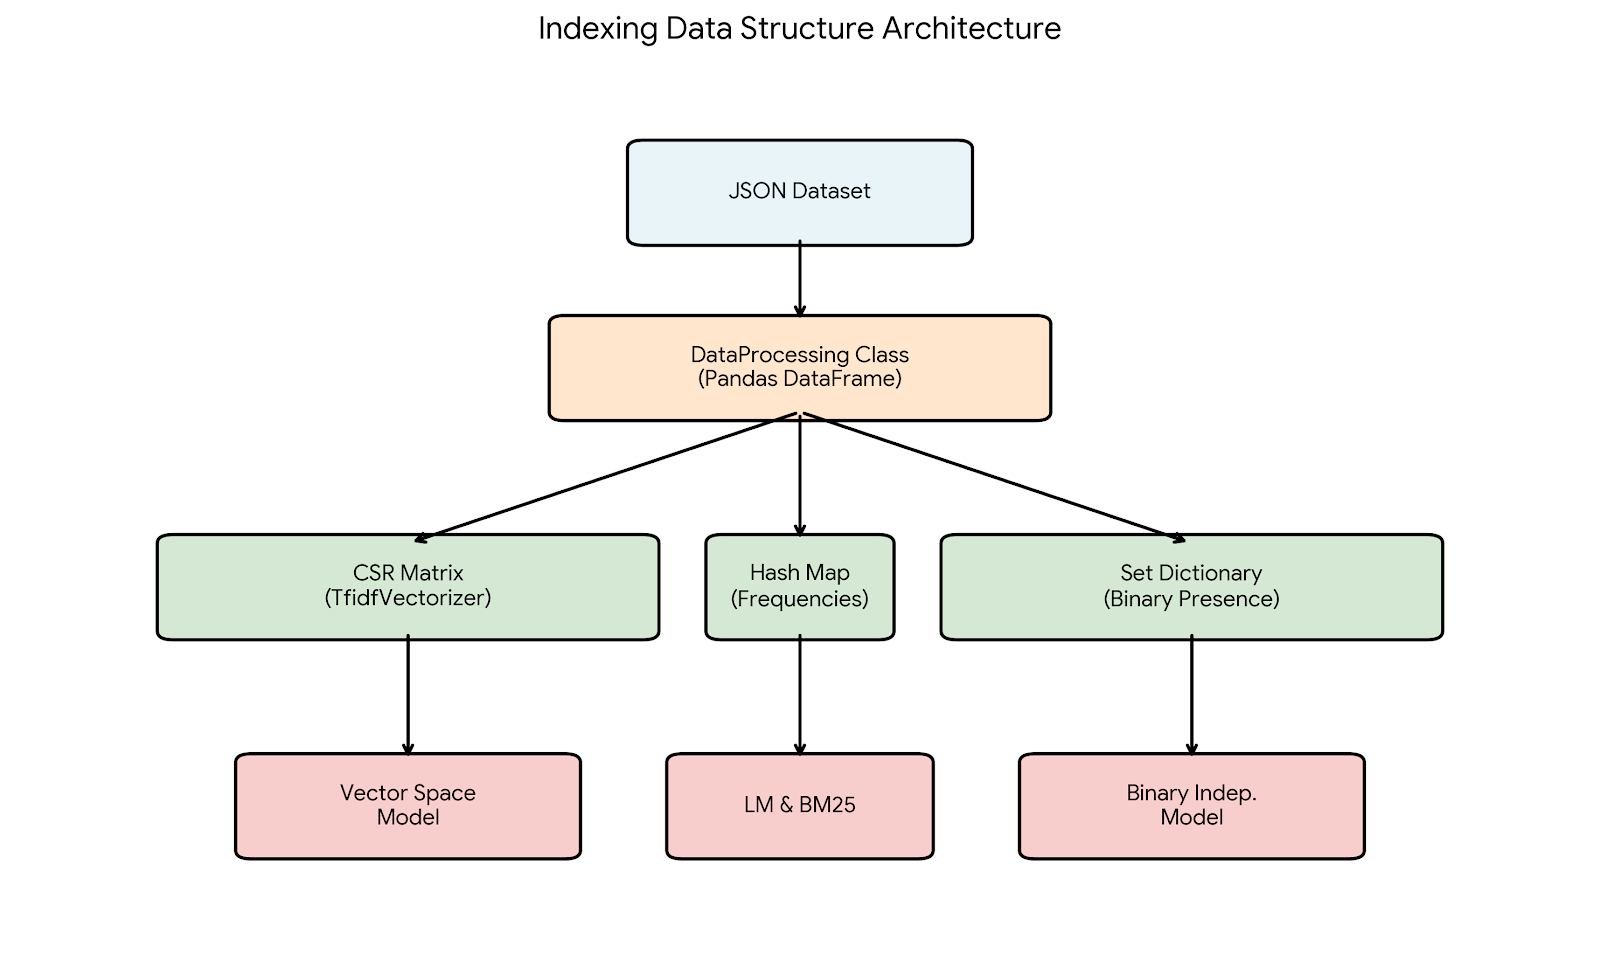
\includegraphics[width=\linewidth]{../eval/figures/indexing_ds.png}
    \caption[Indexing Data Structure Architecture]{
        Index design process for the implemented retrieval models. All 
        retrieval models share the same dataset. 
    }
    \label{figure:indexing}
\end{figure}